\documentclass[10pt,twocolumn,letterpaper]{article}

\usepackage{cvpr}
\usepackage{times}
\usepackage{epsfig}
\usepackage{graphicx}
\usepackage{amsmath}
\usepackage{amssymb}

% Include other packages here, before hyperref.

% If you comment hyperref and then uncomment it, you should delete
% egpaper.aux before re-running latex.  (Or just hit 'q' on the first latex
% run, let it finish, and you should be clear).
\usepackage[breaklinks=true,bookmarks=false]{hyperref}

\cvprfinalcopy % *** Uncomment this line for the final submission

\def\cvprPaperID{****} % *** Enter the CVPR Paper ID here
\def\httilde{\mbox{\tt\raisebox{-.5ex}{\symbol{126}}}}

% Pages are numbered in submission mode, and unnumbered in camera-ready
%\ifcvprfinal\pagestyle{empty}\fi
\setcounter{page}{1}
\begin{document}

%%%%%%%%% TITLE
\title{CSC 449: Machine Vision Project
\\ Real Time Facial Emotion Recognition (MobileNet vs ShuffleNet)
\\Team: AID
}

\author{Aeshaan Wahlang\\
Dept. Computer Science\\
{\tt\small awahlang@ur.rochester.edu}
% For a paper whose authors are all at the same institution,
% omit the following lines up until the closing ``}''.
% Additional authors and addresses can be added with ``\and'',
% just like the second author.
% To save space, use either the email address or home page, not both
\and
Daniel Barnett\\
Dept. Computer Science\\
{\tt\small dbarnette@ur.rochester.edu}
\and
Ivanah Tannica Desoloc\\
Ain Center for Entrepreneurship\\
{\tt\small desoloc@ur.rochester.edu}
}

\maketitle
%\thispagestyle{empty}

%%%%%%%%% ABSTRACT
\begin{abstract}
   We compare two efficient convolutional neural networks architectures specially developed for mobile devices with limited computing power. The first architecture, MobileNets, is based on a streamlined architecture that uses depth-wise separable convolutions to build light weight deep neural networks. The second architecture, ShuffleNet, improves on the former by utilizing two new operations, pointwise group convolution and channel shuffle, to greatly reduce computation cost while maintaining accuracy. Upon completion, we developed a real-time face detection and emotion classification system that can run on low-end devices.
\end{abstract}

%%%%%%%%% BODY TEXT
\section{Introduction}

Many real world applications such as robotics, self-driving car, and augmented reality require recognition tasks to be carried out in a timely fashion, but usually on computationally limited platforms. To meet this need, two recent papers MobileNets [2] and ShuffleNet [3] propose efficient models for vision applications in such circumstances. We have performed a comparative study on the two models using the AffectNet [1] database for real time facial emotion recognition.

%-------------------------------------------------------------------------

\section{Related works}
Andrew G. Howard et. al. [1] developed a class of efficient convolutional neural network models for mobile and embedded vision applications called MobileNets. Their model is based on a streamlined architecture that uses depth-wise separable convolutions, a form of factorized convolutions to build a lightweight deep neural network. The depth-wise separable convolutions are made up of two layers: depth wise convolutions and pointwise convolutions. The latter, is extremely efficient relative to standard convolution. However, it only filters input channels, it does not combine them to create new features. To do this, they added an additional layer i.e. the pointwise convolution, that computes linear combination of the outputs of the depth wise convolutions via 1x1 convolution. To further increase efficiency, they introduce two global hyper-parameters. A width multiplier \(\alpha\), which thins the network uniformly at each layer, and resolution multiplier \(\rho\), which reduces the computational cost of the network. These hyper-parameters allow the model builder to choose the right sized model for their application, in a trade off with accuracy. They demonstrate the effectiveness of the model with a variety of application, from object recognition to facial feature recognition.

Xiangyu Zhang et. al [2] developed a similar model, that is based on a new architecture that utilizes two new operations, pointwise group convolution and channel shuffle, to greatly reduce computation cost while maintaining accuracy. The former reduces computation complexity of 1x1 convolution. To overcome the side effects brought by group convolution (i.e. if multiple group convolutions stack together, outputs from a certain channel are only derived from a small fraction of input channels), the latter is introduced to help the information flowing across feature channels. Based on the two techniques, they have built a highly efficient architecture called ShuffleNet. Compared to traditional convolutional neural networks, for a given computation complexity budget, ShuffleNet allows more feature map channels, which helps to encode more information and is especially critical to the performance of very small networks.



%-------------------------------------------------------------------------
\subsection{Data Preprocessing}

The data we use to train our models for this project come from the AffectNet dataset [3]. The dataset consist of facial expression images that have been uniquely labeled into 8 different emotions, Anger, Contempt, Disgust, Fear, Happy, Neutral, Sad and Surprise. These emotions were based on the intensity of valence and arousal (dimensional model). The dataset consist of over 1 million images, however about 440,000 images were manually annotated. Our models were trained only on the manually annotated images.
Each image was then resized to 224 x 224. The number of images labeled ‘Happy’ and “Neutral” in the dataset was much larger than any class about 3 times as many. To reduce the chances of overfitting, were generated mirror images for each of the other emotions in an effort to increase the number of images. We then reduced the number of images in the ‘Happy’  and ‘Neutral’ so that the outnumber the other classes by a maximum of 5000 images.
An 80:20 split was then done on this set of images, to create the training set(1,82,576 images) and the testing set(45,644) images). A segregated test set which consisted a 100 randomly sampled images from each class was also created. 


%-------------------------------------------------------------------------
\subsection{Facial Detection}

To detect faces in video frames, we used the Viola-Jones object detection framework through OpenCV. The algorithm was picked for its 3 important characteristics:
\begin{itemize}
  \item Robust - very high detection rate and very low false-positive rate
  \item Real-time - for practical applications, at least 2 frames per second must be processed
  \item Efficient and lightweight - doesn’t require a lot of resources
\end{itemize}

The algorithm has 4 stages:
\begin{enumerate}
  \item Haar feature selection
  \item Creating an Integral Image
  \item Adaboost Training
  \item Cascading Classifiers
\end{enumerate}


%-------------------------------------------------------------------------

\section{Methodology}

\subsection{MobileNets Model}

Our MobileNet model was built from scratch and trained on the PyTorch library. The depthwise convolutions were built using group convolutions for each layer where the number of groups were equal to the number of inputs to that layer. This effectively convolved a single filter with a single input. The pointwise convolutions layer were created using filters of size 1x1 and followed every depthwise convolution layer.

We experimented with various network structures, training them with a subset of our training set for 4 epochs and measuring their performance on a subset of the test set. This was done to find the optimum network structure, which is described in Table 1





\begin{center}
\begin{tabular}{ |c|c|c| } 
 \hline
 Network Layers & Output Size & Kernel Stride \\ 
 \hline
 Conv & (122,122,32) & 2 \\
 \hline
 Conv-DW  & (122,122,64) & 1 \\ 
 \hline
 Conv-DW & (56,56,128) & 2 \\ 
 \hline
 Conv-DW & (56,56,128) & 1 \\ 
 \hline
 Conv-DW & (28,28,256) & 2 \\ 
 \hline
 Conv-DW & (28,28,256) & 1 \\ 
 \hline
 Conv-DW & (14,14,512) & 1 \\ 
 \hline
 Conv-DW & (14,14,512) & 1 \\ 
 \hline
 Conv-DW & (7,7,1024) & 1 \\ 
 \hline
 Conv-DW & (1,1,1024) & 2 \\ 
 \hline
 Linear & 1024 & - \\ 
 \hline
 Linear & 100 & - \\ 
 \hline
 Linear & 8 & - \\ 
 \hline
\end{tabular}
\end{center}

Every Depthwise convolution layer in followed by a pointwise convolution layer. All the layers are followed by a ReLU activation layer and the final Linear layer uses a Softmax activation. The mobile architecture does not use Maxpool layers and image subsampling is achieved through strided kernels. Each layer that is not a Point wise convolution layer uses a 3x3 kernel. The model uses a Cross Entropy loss function with Stochastic Gradient Descent optimizer. A dynamic learning rate was used which started at 0.01 and dropped by a factor of 10 after 10 epochs to a final rate of 0.0001. 
The total number of trainable parameters in the model is  3,260,600 with a memory requirement of 13.20 MegaBytes.   

\subsection{ShuffleNet Model}
Like MobileNets we chose to implement the ShuffleNet model ourselves using the PyTorch framework. The benefit of ShuffleNet is that we are able to create a network with many more layers than MobileNets, but with reduced computational complexity. This is due to the use of channel shuffles in the pointwise group convolutions. We trained the model on the recommended network structure in the original paper with a group number of 3.

\begin{figure}[ht]
\caption{ShuffleUnit with a kernel stride of 1 and a kernel stride of 2 [3]}
\centering
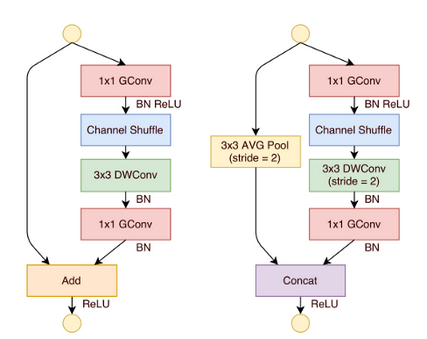
\includegraphics[width=0.35\textwidth]{shuffleunit}
\end{figure}


\begin{figure}[ht]
\caption{Recommended ShuffleNet network in original paper [3]}
\centering
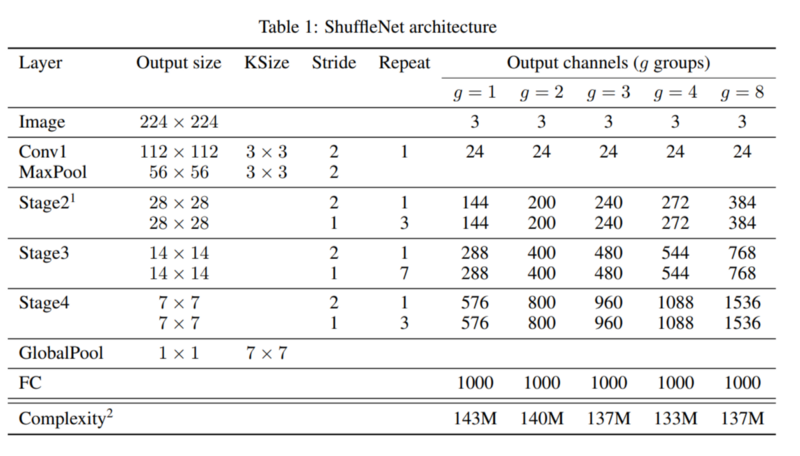
\includegraphics[width=0.5\textwidth]{shufflenet}
\end{figure}

\subsection{Model Training}
Both the MobileNet and ShuffleNet models were trained on the training set for 40 epochs on CIRC Bluehive.

\section{Experiments \& Results}

\subsection{Performance on Test Set}
The performance of both our models on the test set of 22,894 randomly sampled images is shown below. It is to be noted that the speed of the models depends on the computational resources available.

\begin{center}
\begin{tabular}{ |c|c|c| } 
 \hline
 - & MobileNets & Shufflenet \\ 
 \hline
 Accuracy & 58\% & 68\% \\
 \hline
 Speed  & 612 Seconds & 548 Seconds \\ 
 \hline
 Memory & 13.20 MB & - \\ 
 \hline
\end{tabular}
\end{center}

\subsection{Performance on Segregated Test Set}

The performance of both our models on the  set of 100  sampled images from each class is shown below.

\begin{figure}[ht]
\caption{Accuracies of each emotion for both models}
\centering
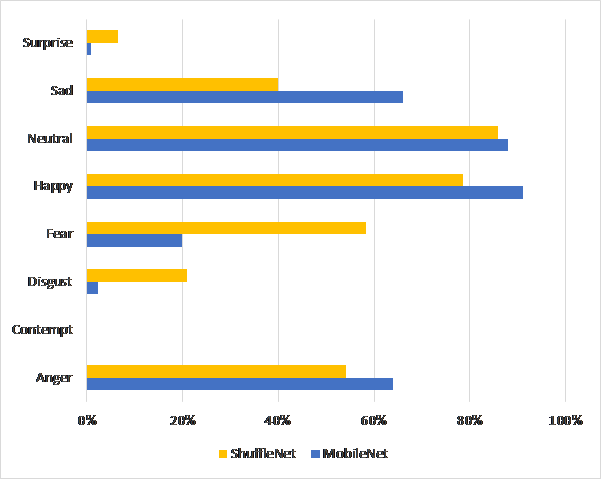
\includegraphics[width=0.4\textwidth]{SegregatedAcc}
\end{figure}

Both the MobileNets model and ShuffleNet model perform well when classifying images of the “Happy”, “Anger”, “Neutral” and “Sad” expressions. However ShuffleNet’s performance drops with the other expressions and MobileNet struggles.
The facial differences between these expressions are more subtle. The classification of many facial features in these expressions tend to overlap with others. For example, facial expressions of Fear look similar to Surprise, while expressions of Contempt are similar to Neutral. The predictions of our models with these expressions are detailed in Figure \#4 .

\begin{figure}[ht]
\caption{Overlap of each emotion using ShuffleNet}
\centering
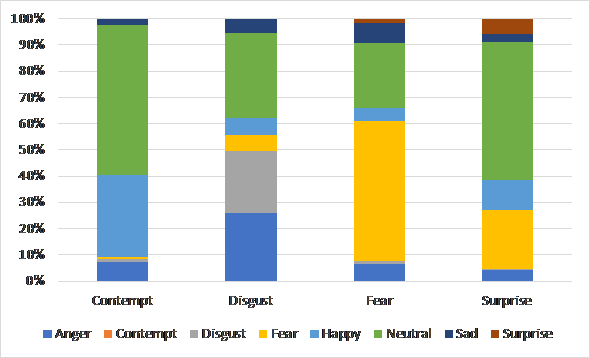
\includegraphics[width=0.4\textwidth]{Predicted}
\end{figure}

\begin{figure}[ht]
\caption{Example images, True class (Predicted Class)}
\centering
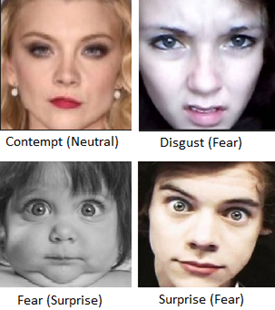
\includegraphics[width=0.3\textwidth]{emotions}
\end{figure}

The differences between these expressions and the predicted expressions are subtle and fine. At first glance, certain cases can be difficult for humans to identify as well.
This suggests that these fine differences are not identified by our models and that the sequence of convolutions that our model performs on the images are not enough to detect such subtle changes.

\subsection{Real Time Performance}
Real time video performance of our models is consistent with the performance on the Test set. The models classify the extracted facial images from the video source in an average of (time here) seconds. The models recognize the expressions, “Anger”, “Happy”, “Neutral” and “Sad” fairly well. However with expressions of “Contempt” and “Disgust”, the models switch between multiple predictions. During our testing, we experienced considerable lag when dealing with more than 2 faces. This is due to computational limitations of our systems and unoptimized facial detection. The Figures \#6, \#7  and \#8 are screenshots of the real time performance.

\begin{figure}[ht]
\caption{Example of happy, neutral, and anger}
\centering
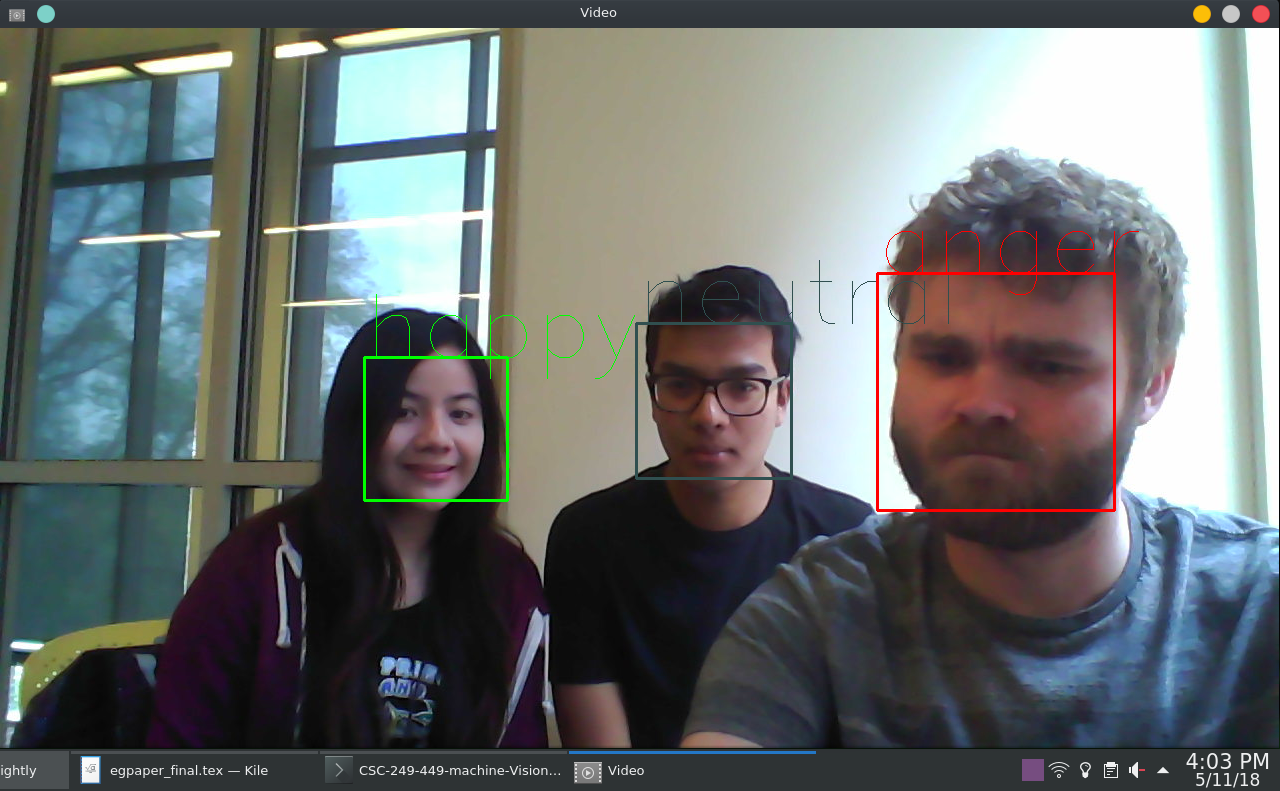
\includegraphics[width=0.4\textwidth]{happy_neutral_angry}
\end{figure}

\begin{figure}[ht]
\caption{Example of fear, surprise, and sadness}
\centering
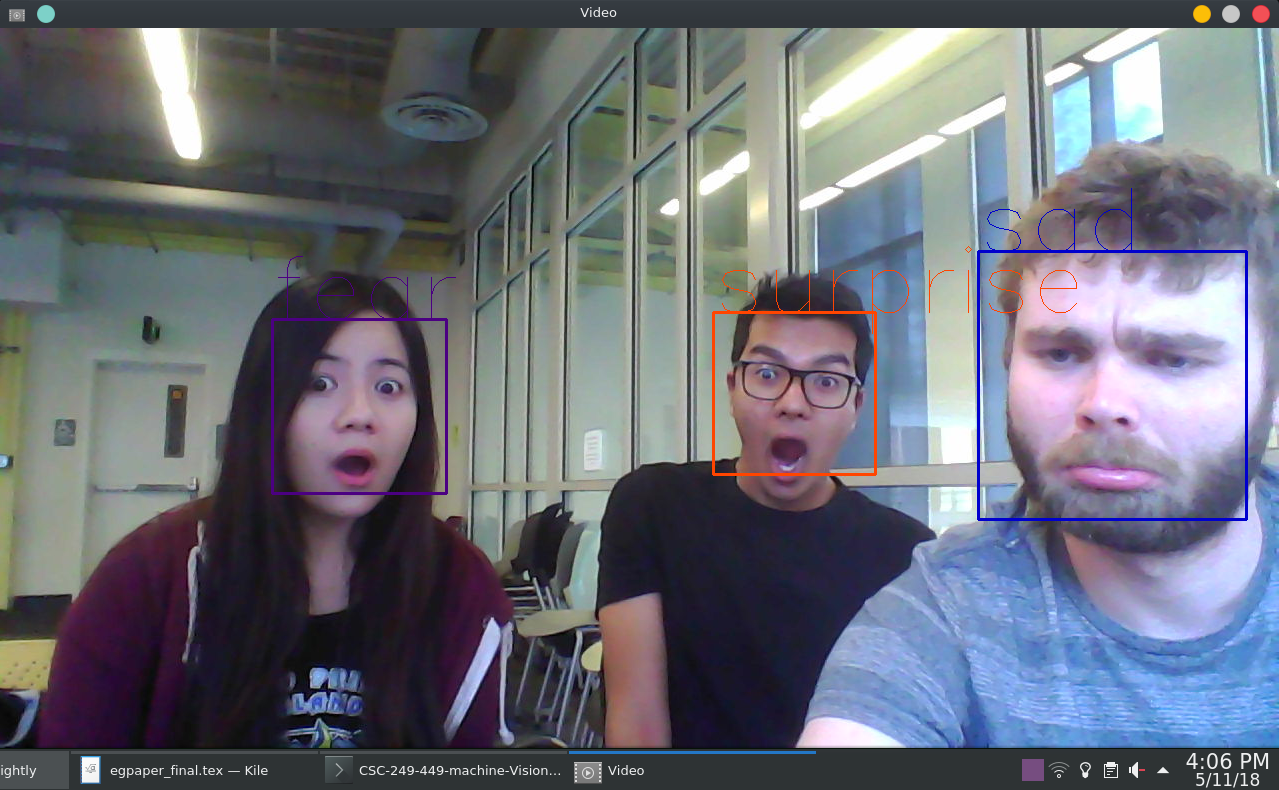
\includegraphics[width=0.4\textwidth]{fear_surprise_sad}
\end{figure}

\begin{figure}[ht]
\caption{Example of disgust and anger}
\centering
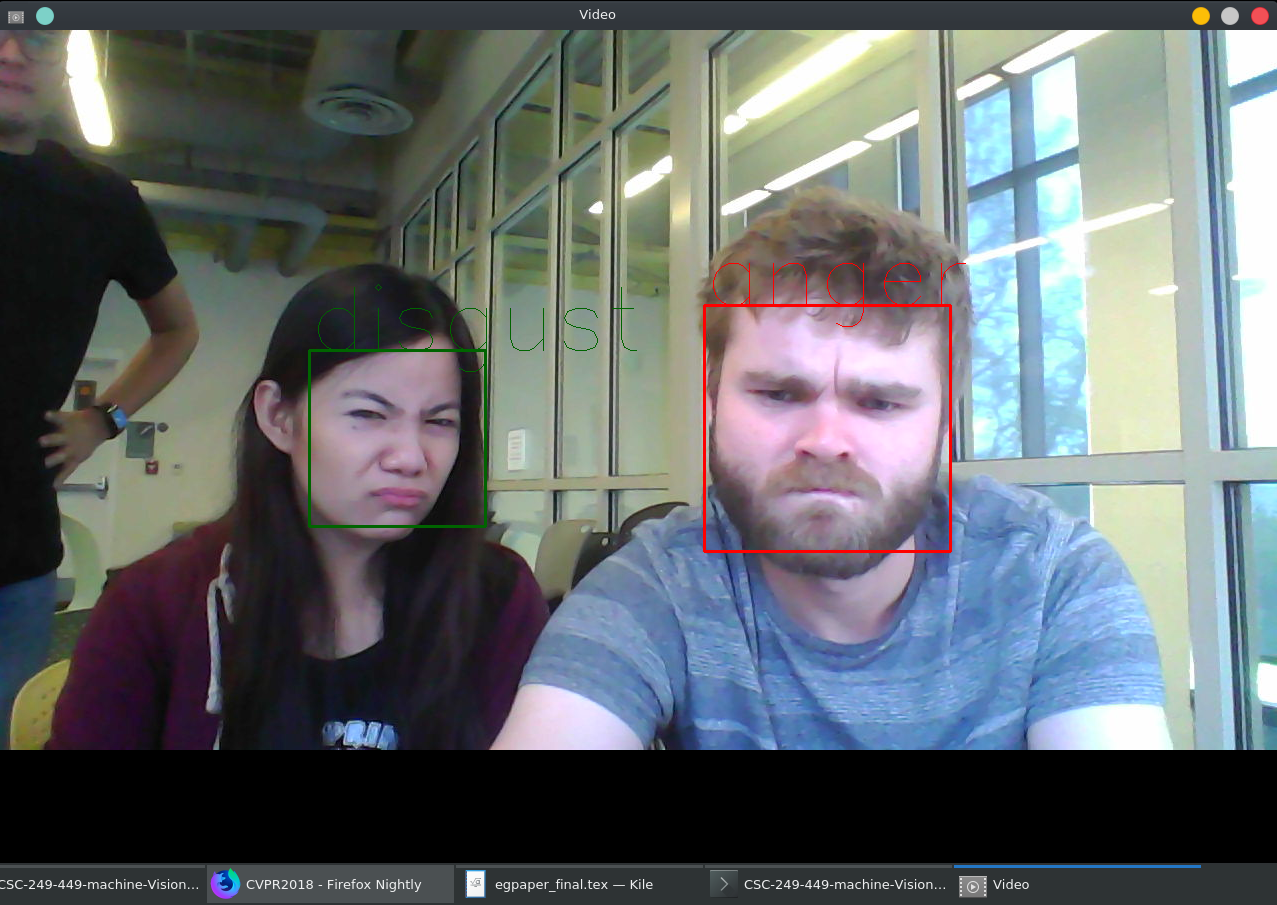
\includegraphics[width=0.4\textwidth]{disgust_anger}
\end{figure}

\subsection{MobileNets vs ShuffleNet}

From our experiments it is clear that with respect to problem of facial emotion recognition, the ShuffleNet architecture significantly performs better than the MobileNet architecture. ShuffleNet even with a smaller number of parameters in the model proves to be more robust and generalizes better. 
We attribute MobileNet’s poorer performance to the following reasons.
 
a) The primary reasons for ShuffleNet’s channel shuffle was to increase cross group information flow between the input channels for multiple convolution layers. Since MobileNet’s depthwise convolutions are only followed by point wise convolutions, we suspect that some  smaller features are overshadowed by larger ones during the 1x1 convolution. While in ShuffleNet, the pointwise convolutions are grouped convolutions, so a filter is not convolved with all the input channels and these smaller features come through.

b) Unlike ShuffleNet, the MobileNet architecture does not use MaxPool layers. Sub-sampling is achieved through strided convolutions. As we know, MaxPool layers create partial translation invariance. This invariance could be the key in differentiating between similar facial expressions such as Fear and Anger. The facial expressions ‘Contempt’, ‘Disgust’, ‘Fear’ and ‘Surprise’ have similarities with other expressions and differ in subtle ways. Because of the absence of MaxPool layers, these subtle differences do not come through even if they are detected in some convolution layer.

MobileNet performed fairly well when detecting ‘Happy’, ‘Angry’, ‘Neutral’ and ‘Sad’, since these expressions have distinct features and differ substantially from each other. However, it struggled with expressions of ‘Fear’, ‘Contempt’, ‘Disgust’ and ‘Surprise’. The reasons above could explain why ShuffleNet performed better at these emotional expressions.

\section{Conclusion}
While MobileNet performed well in identifying 4 emotions, ShuffleNet channel shuffle and MaxPool layers give it the edge. The ShuffleNet model comfortably detects 6 out of the 8 emotions and proves to be more robust and efficient than the MobileNet model.
However, the problem of facial emotion recognition requires the detection of small, subtle changes in facial features and neither of these models alone would suffice.

\section{Future Work}
To increase the accuracy of the emotion recognition, classification modes could be built just for specific facial features such as the eyes or lips. These can then be used to as inputs to another model that would classify the facial emotion.
Further improvements to the current network structures such as adding MaxPool layers to the MobileNet model could improve its performance as well.


{\small
\bibliographystyle{ieee}



\begin{thebibliography}{9}

\bibitem{affectnet} 
Ali Mollahosseini, Behzad Hasani, Mohammad H. Mahoor
\textit{ AffectNet: A Database for Facial Expression, Valence, and Arousal Computing in the Wild}. 
9 Oct 2017.

\bibitem{mobilenets} 
Andrew G. Howard, Menglong Zhu, Bo Chen, Dmitry Kalenichenko, Weijun Wang, Tobias Weyand, Marco Andreetto, Hartwig Adam
\textit{MobileNets: Efficient Convolutional Neural Networks for Mobile Vision Applications}. 
April 2017.

\bibitem{shufflenet} 
Xiangyu Zhang, Xinyu Zhou, Mengxiao Lin, Jian Sun
\textit{ShuffleNet: An Extremely Efficient Convolutional Neural Network for Mobile Devices}. 
7 Dec 2017.
 

\end{thebibliography}



}

\end{document}
